\chapter{Proof of Concept}
\label{ch:proof-of-concept}
Dit hoofdstuk bevat het vergelijkend experiment tussen twee eerder gekozen open source serverless (FaaS) frameworks, namelijk Fission en OpenFaaS. In dit onderdeel worden de twee frameworks opgezet op een Kubernetes cluster die bestaat uit één node. Beide frameworks worden opgezet op een MacBook Pro waarop Minikube draait. Minikube is een ''Out-of-the-box'' Kubernetes cluster die overal kan draaien. Er wordt gekozen om gebruik te maken van Minikube omdat op deze manier beide frameworks op identiek dezelfde hardware kunnen gedraaid worden. Daarnaast biedt Minikube dezelfde functionaliteiten als een volledige Kubernetes cluster die elders is opgezet. Dit hoofdstuk is opgedeeld in twee grote onderdelen waarbinnen telkens dezelfde secties met dezelfde stappen voor elk framework terug te vinden zijn. Daarnaast is er eveneens een sectie in dit hoofdstuk terug te vinden waarin de demo functie die serverless gedraaid zal worden op de frameworks wordt voorgesteld. De demo bestaat uit het deployen van een Python functie die de functionaliteit van beide frameworks demonstreert en de executietijd van de functie meet. Later wordt er in dit onderzoek een vergelijking tussen Fission en OpenFaaS gemaakt waarbij onder meer gekeken zal worden naar het verschil in executietijd tussen de geschreven functie alsook de gebruiksvriendelijkheid. Deze Proof of Concept moet meer inzicht geven in beide frameworks en geeft een duidelijk beeld van wat deze precies inhouden.
\\\\
\section{Voorbereiding omgeving}
\label{sec:voorbereiding-omgeving}
\subsection{Onderliggende hardware}
Het experiment zal worden uitgevoerd op een MacBook Pro, model 2018 met volgende specificaties:
\begin{itemize}
    \item Processor: 2,2 GHz Intel Core i7
    \item Memory: 16 GB 2400 MHz DDR4
    \item Graphics: Radeon Pro 555X 4 GB en Intel UHD Graphics 630 1536 MB
    \item Opslag: 256 GB SSD
\end{itemize}

\subsection{Packet manager}
Om de opstelling van het experiment klaar te zetten is het zinvol gebruik te maken van Homebrew\footnote{https://brew.sh/}, dit is een packetmanager ontwikkeld voor macOS. Homebrew zorgt ervoor dat softwarepakketten kunnen worden gedownload uit bestaande repositories. In de verdere uitwerking van dit onderzoek wordt Homebrew eveneens gebruikt voor het installeren van software.\\\\
Homebrew kan worden geïnstalleerd door volgend commando in de Terminal uit te voeren: 
\begin{lstlisting}[language=bash]
$ /usr/bin/ruby -e "$(curl -fsSL 
https://raw.githubusercontent.com/Homebrew/install/master/install)"
\end{lstlisting}

\subsection{Softwarepakketten}
Alvorens de frameworks kunnen worden opgezet moeten er reeds enkele softwarepakketten aanwezig zijn. Enerzijds is Docker nodig als container engine, anderzijds Kubernetes als container platform. Daarnaast is er ook een hypervisor nodig die het draaien van een Minikube cluster mogelijk maakt. In dit onderzoek wordt gebruik gemaakt van VirtualBox als hypervisor, deze is open source en gratis. De softwarepakketten kunnen als volgt geïnstalleerd worden met Homebrew:        
\begin{lstlisting}[language=bash]
$ brew tap caskroom/cask
$ brew cask install virtualbox
$ brew cask install docker
$ brew cask install minikube
$ brew install kubernetes-cli
\end{lstlisting}

\section{Python demofunctie}
\label{sec:python-demofunctie}
Aan de hand van een zelfgeschreven Python functie zal de werking van beide frameworks worden gedemonstreerd. De demofunctie is eenvoudig en bestaat uit een print statement dat de gebruiker verwelkomt, vervolgens wordt er een loop uitgevoerd die ervoor zorgt dat de functie toch even loopt en uiteindelijk wordt deze uitvoeringstijd weggeschreven naar een Google Spreadsheet bestand. De Python functie maakt gebruik van de Google API voor het wegschrijven naar het spreadsheet bestand. De functie wordt verpakt in een Docker image zodat deze naadloos kan worden gedeployed op beide frameworks. De Docker image met de functie is gepubliceerd op de Docker Hub repository van Lennert Mertens (private repository). Om gebruik te kunnen maken van Google spreadsheets moet er een Google project worden aangemaakt via de Google API, deze stappen staan verder beschreven. Er wordt gekozen voor dit soort functie zodat er later in dit onderzoek een besluit kan worden gevormd over welk framework de snelste executie van functies biedt. Het ultieme doel is dat de data in het Google bestand kan worden geanalyseerd en vergeleken. Elke demo start met een leeg werkblad zodat de resultaten die werden weggeschreven toepasbaar zijn op het specifieke framework dat werd getest.

\subsection{Google API}
De Python functie schrijft de executietijd van de functies weg naar een bestand op Google spreadsheets. Om gebruik te maken van een spreadsheet bestand moet eerst de API worden geconfigureerd, daarnaast moeten ook de credentials op de demo machine worden geconfigureerd. Het Goolge project wordt opgezet zodat de functie data kan wegschrijven naar de spreadsheet, in sectie \ref{sec:google-api} is een gedetailleerd stappenplan terug te vinden voor het instellen van de Google API in combinatie met Google spreadsheets. Om gebruik te maken van Google API features moeten oauth2client, gspread en google-api-python-client geïnstalleerd worden. De drie packages die nodig zijn voor de uitvoer van de functie worden gebundeld in een tekstbestand ''requirements.txt'', dit bestand kan vervolgens door ''pip'' worden gebruikt voor de installatie van de softwarepakketten, het bestand is terug te vinden in bijlage \ref{sec:requirements.txt}.

\newpage
\subsection{Code demofunctie}
\begin{lstlisting}[language=python]
import time
import gspread
from oauth2client.service_account import ServiceAccountCredentials

# Function to get the first empty row in Gooogle Spreadsheet
def next_available_row(worksheet):
      str_list = filter(None, worksheet.col_values(1)) 
      return str(len(str_list)+1)

# Initialize variables for Google API
scope = ['https://spreadsheets.google.com/feeds',
         'https://www.googleapis.com/auth/drive']
credentials = ServiceAccountCredentials
              .from_json_keyfile_name('credentials.json', scope)
client = gspread.authorize(credentials)
worksheet = client.open("executietijd-openfaas").sheet1
next_row = next_available_row(worksheet)

# Start timer 
start = time.time()

# Print message visible by users
print("Hello everyone, this is a serverless demo function!")

# Start loop function to measure execution time
a = range(1000000)
b = []
for i in a:
     b.append(i*2)

# Stop timer
end = time.time()

# Calculate the execution time of the function in seconds
execution_time= end - start

# Write the execution time to Google spreadsheet
worksheet.update_acell("A{}".format(next_row), execution_time)
\end{lstlisting}


\section{OpenFaaS}
Het eerste framework dat wordt uitgetest is OpenFaaS. Het experiment wordt opgezet op een MacBook Pro die voldoet aan voorgaande specificaties en beschikt over de benodigde softwarepakketten zoals eerder ook beschreven werd. De stappen die doorlopen worden in het opzetten en uitvoeren van het experiment, zijn steeds duidelijk gedocumenteerd en staan chronologisch gerangschikt. De installatieprocedure is eenvoudig te volgen en is reproduceerbaar aan de hand van de gedocumenteerde stappen en bijhorende scripts.

\subsection{Configuratie Minikube}
Vooraleer OpenFaaS geïnstalleerd kan worden, wordt er een lokale Kubernetes cluster die bestaat uit één node opgezet met Minikube. Een Minikube cluster biedt dezelfde functionaliteiten als een productieomgeving waarop een Kubernetes cluster is geïnstalleerd. Er wordt gebruik gemaakt van Kubernetes als container orchestrator. Een orchestrator is een tool die instaat voor het management van containers en microservice applicaties. Kubernetes zorgt ervoor dat applicaties schaalbaar kunnen worden opgezet, staat in voor het volledige beheer van de containers en voorziet ''High-availability''.
\\
In sectie \ref{sec:voorbereiding-omgeving} werden de benodigde softwarepakketten reeds geïnstalleerd. Indien alle stappen succesvol werden doorlopen dan kan de Minikube cluster probleemloos als volgt worden gestart. Na de installatie wordt eerst ook de status van de cluster nagegaan.

\begin{lstlisting}[language=bash]
$ minikube start
$ minikube status
\end{lstlisting}

De uitvoer van het tweede commando geeft een overzicht dat er als volgt zou moeten uitzien, het IP adres wijkt mogelijks af van hetgene in de output. Wanneer de output overeenkomt met deze dan is Minikube succesvol geïnstalleerd.
\begin{lstlisting}[language=bash]
host: Running
kubelet: Running
apiserver: Running
kubectl: Correctly Configured: pointing to \ 
minikube-vm at 192.168.99.107
\end{lstlisting}

\subsection{Installatie OpenFaaS}
Indien de installatie van Minikube uit voorgaande sectie succesvol is, dan kan OpenFaaS worden geïnstalleerd. De installatie van OpenFaaS bestaat uit enkele stappen die werden omgevormd tot een shell script. Het is mogelijk dit script vanuit de Terminal uit te voeren, vervolgens start de installatie van OpenFaaS. De volledige installatie van het framework is geautomatiseerd en reproduceerbaar. Het script is terug te vinden als bijlage \ref{sec:installatie-openfaas} onder de naam Installatiescript OpenFaaS. De installatie is gebaseerd op een blogpost van \textcite{Ellis2017}, de founder van OpenFaaS. In de documentatie van OpenFaaS\footnote{https://docs.openfaas.com/} wordt eveneens naar deze blogpost gerefereerd als installatiehandleiding. Na de  uitvoering van het script is OpenFaaS geïnstalleerd bovenop de Minikube cluster. Na de installatie worden enkele artefacten geproduceerd die communicatie met het framework mogelijk maken.
\\
\begin{itemize}
    \item OpenFaaS UI standaard poort: 31112
    \item OpenFaaS UI URL: http://MINIKUBE-IP:31112/ui/
\end{itemize}
 
\subsection{Gebruik OpenFaaS}
\subsubsection{User Interface}
Na de installatie is het mogelijk naar de OpenFaaS UI te surfen, \\bijvoorbeeld: http://192.168.99.107:31112. 
De eerste keer dient er aangemeld te worden met gebruiker ''admin'' (Deze gebruiker wordt aangemaakt in het installatiescript) en het wachtwoord dat in de Terminal werd weergegeven door het installatiescript. Na het aanmelden is de interface zoals in figuur \ref{fig:openfaas-ui} te zien. De UI ziet er vrij sober uit na installatie, er is eveneens een mogelijkheid om een nieuwe functie te deployen via de ''Deploy New Function'' knop. Wanneer gebruikers kiezen een nieuwe functie te deployen dan kunnen ze enerzijds kiezen voor een community functie, dit zijn reeds bestaande functies die op het OpenFaaS framework kunnen gedraaid worden. Anderzijds kunnen gebruikers ook manueel zelfgeschreven functies deployen aan de hand van deze interface. In dit onderzoek worden functies gedeployed via de command line met het faas-cli commando. Deployments van functies via de command line biedt een betere reproduceerbaarheid en is vaak sneller en makkelijker te reproduceren. Er wordt ook bewust gekozen voor de command line tools omdat niet alle serverless frameworks over een UI beschikken. De interface is een leuke feature en is makkelijk in gebruik voor mensen die aan de slag willen met serverless, deze wordt eveneens standaard meegeïnstalleerd met OpenFaaS.
\begin{figure}
    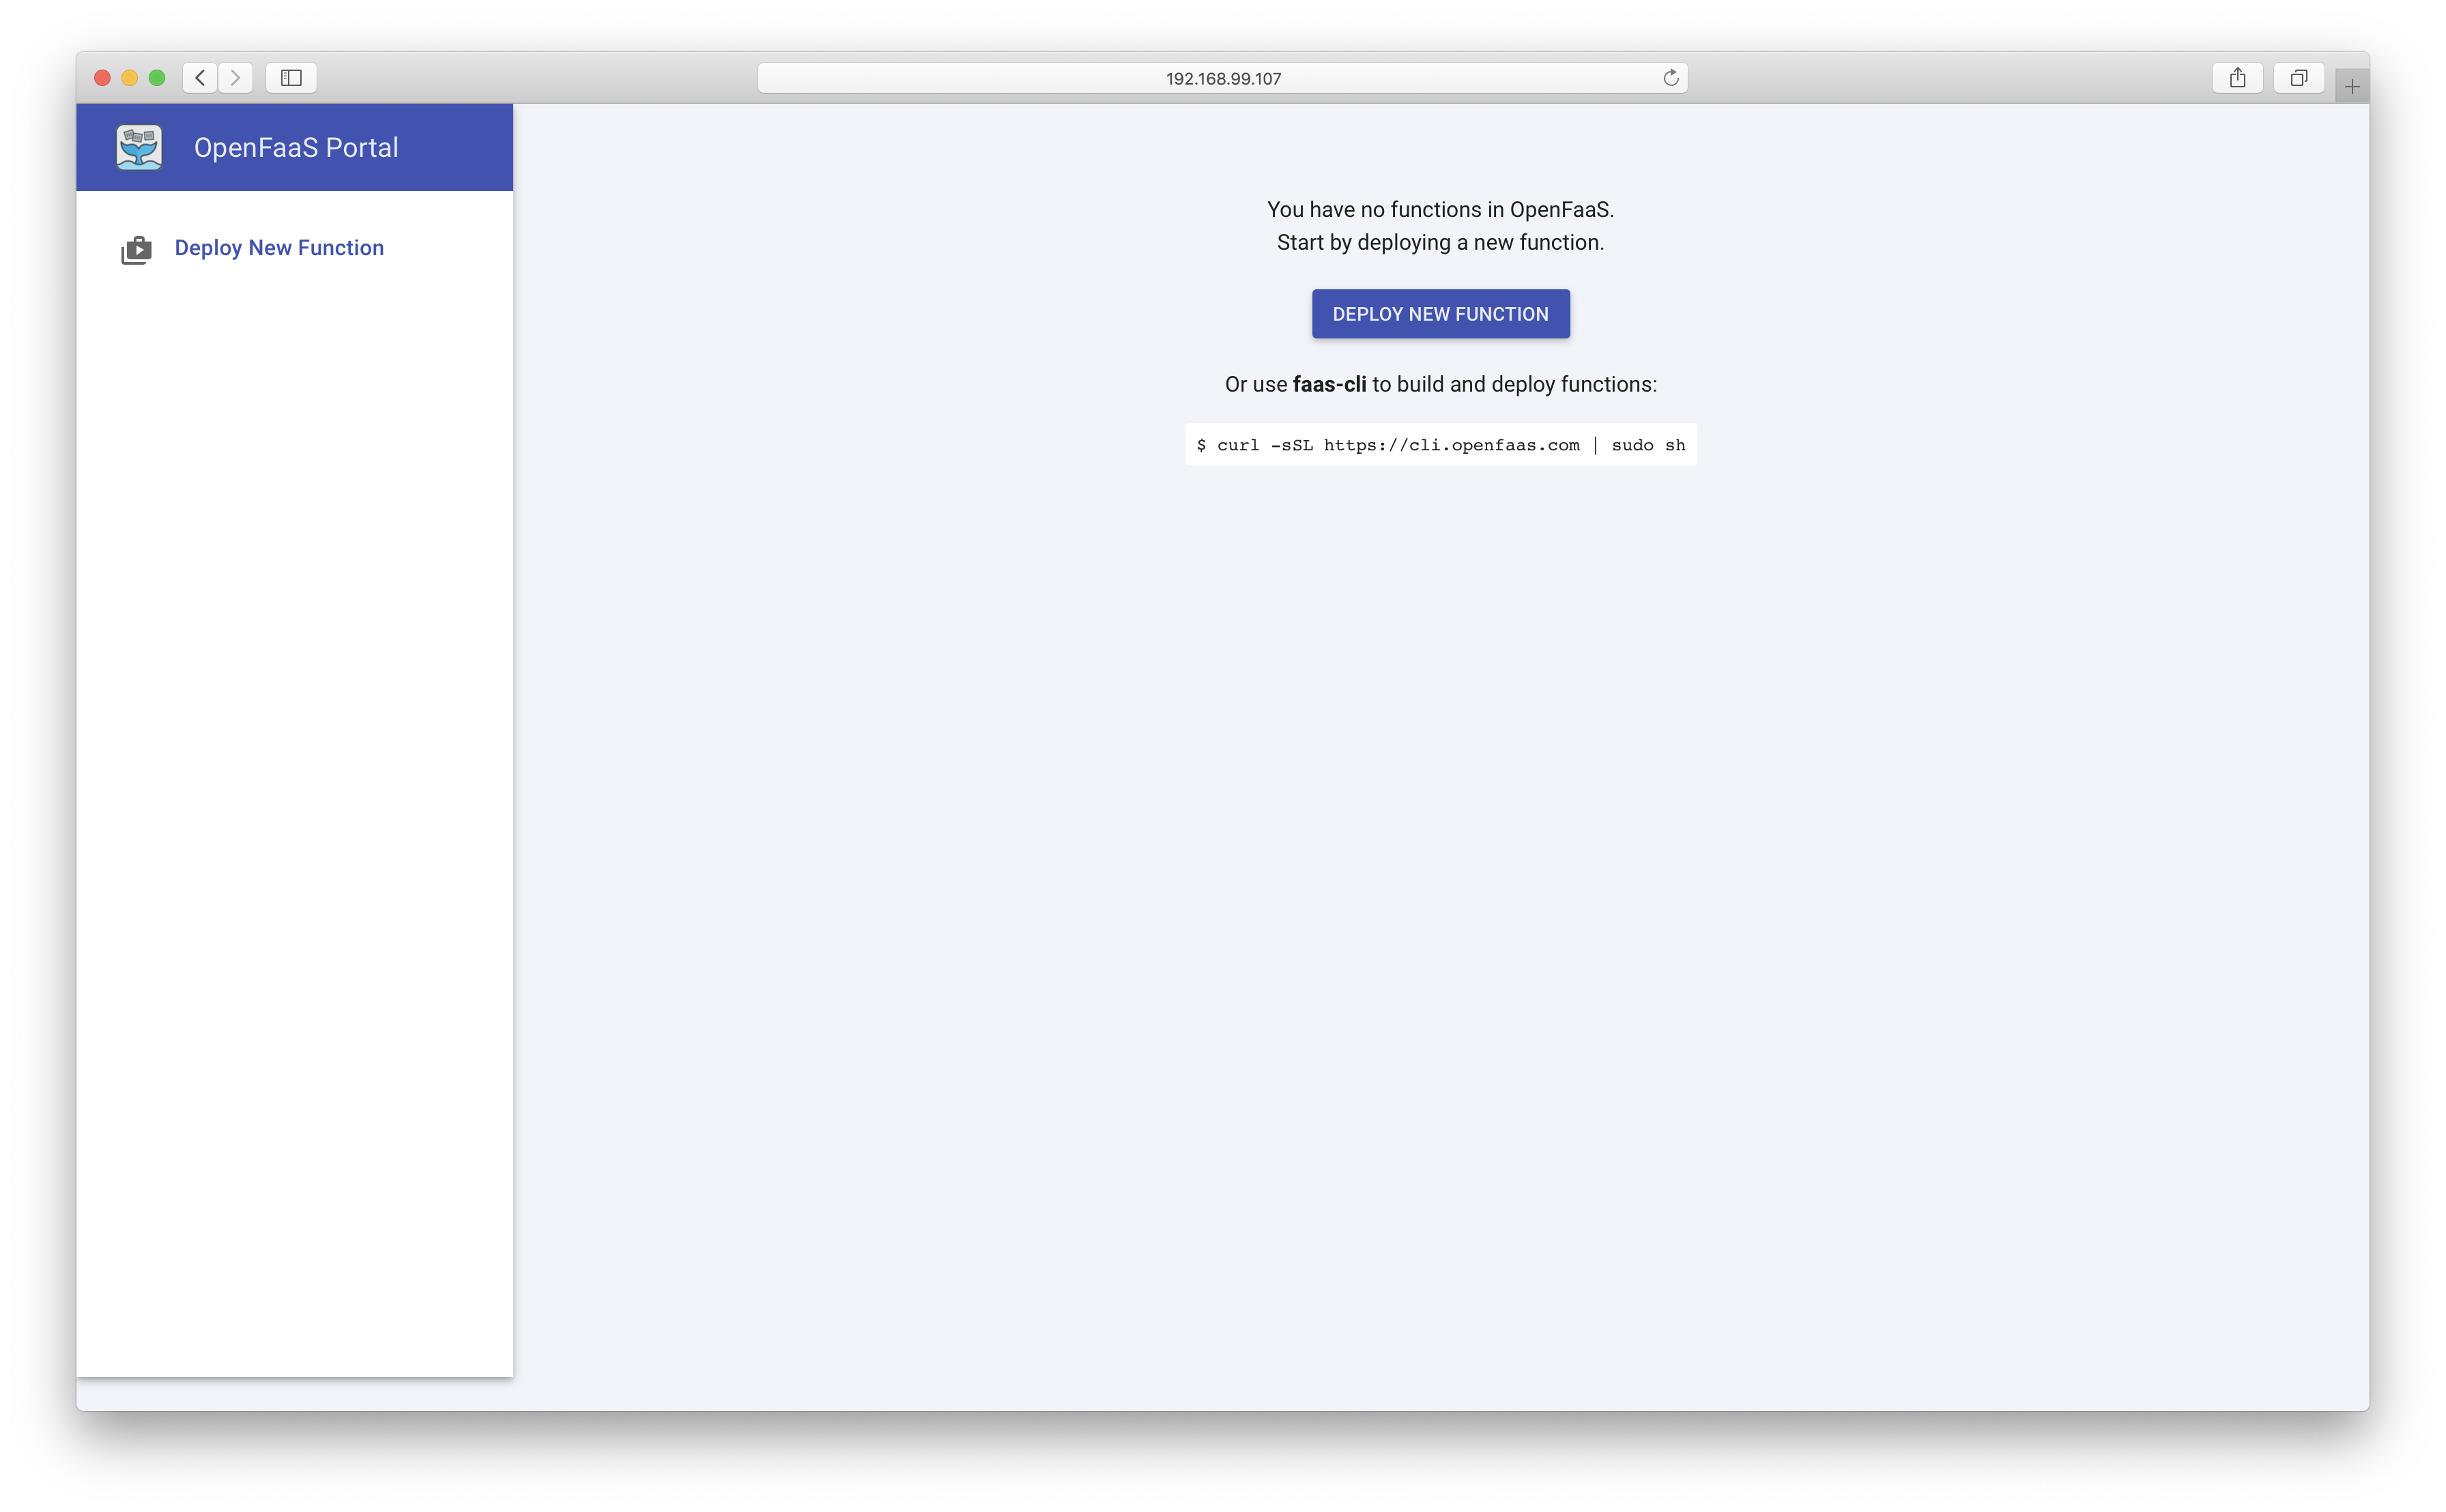
\includegraphics[width=1\textwidth]{img/openfaas-ui.png}
    \caption{OpenFaaS User Interface}
    \label{fig:openfaas-ui}  
\end{figure}

\subsubsection{Command line tools}
Faas-cli is de command line tool die beheer van OpenFaaS voorziet aan de hand van de console. Vooraleer van start te kunnen gaan moet de gebruiker inloggen via de Terminal door volgend commando in te voeren. Het paswoord werd tijdens de installatie in de Terminal weggeschreven, net zoals het IP adres waarop OpenFaaS draait. Daarnaast beschikt de shell ook over environment parameters met het wachtwoord en de URL voor OpenFaaS.
\begin{lstlisting}[language=bash]
$ faas-cli login -g http://$OPENFAAS_URL -u admin -p $PASSWORD
\end{lstlisting}
De command line tools voorzien meer functionaliteiten dan de UI. Het is mogelijk om functies te deployen via de CLI, de omgeving te beheren, confidentiële sleutels en wachtwoorden te beheren etc.

\subsubsection{Prometheus monitoring}
OpenFaaS voorziet monitoring aan de hand van Prometheus, via een Grafana dashboard kunnen verschillende metrics van functies worden bekeken. De configuratie van het dashboard werd reeds voorzien in installatiescript \ref{sec:installatie-openfaas}. Na de configuratie van Prometheus en Grafana kan het dashboard worden geraadpleegd via de GRAFANA\_URL, bijvoorbeeld http://192.168.99.107:32548/dashboard/db/openfaas. In figuur \ref{fig:grafana-dashboard} is het Grafana dashboard zichtbaar dat wordt weergegeven bij het openen van de link. Alvorens dit scherm kan geraadpleegd worden dient de gebruiker in te loggen met de standaard gebruiker ''admin'' met wachtwoord ''admin''.
\begin{figure}
    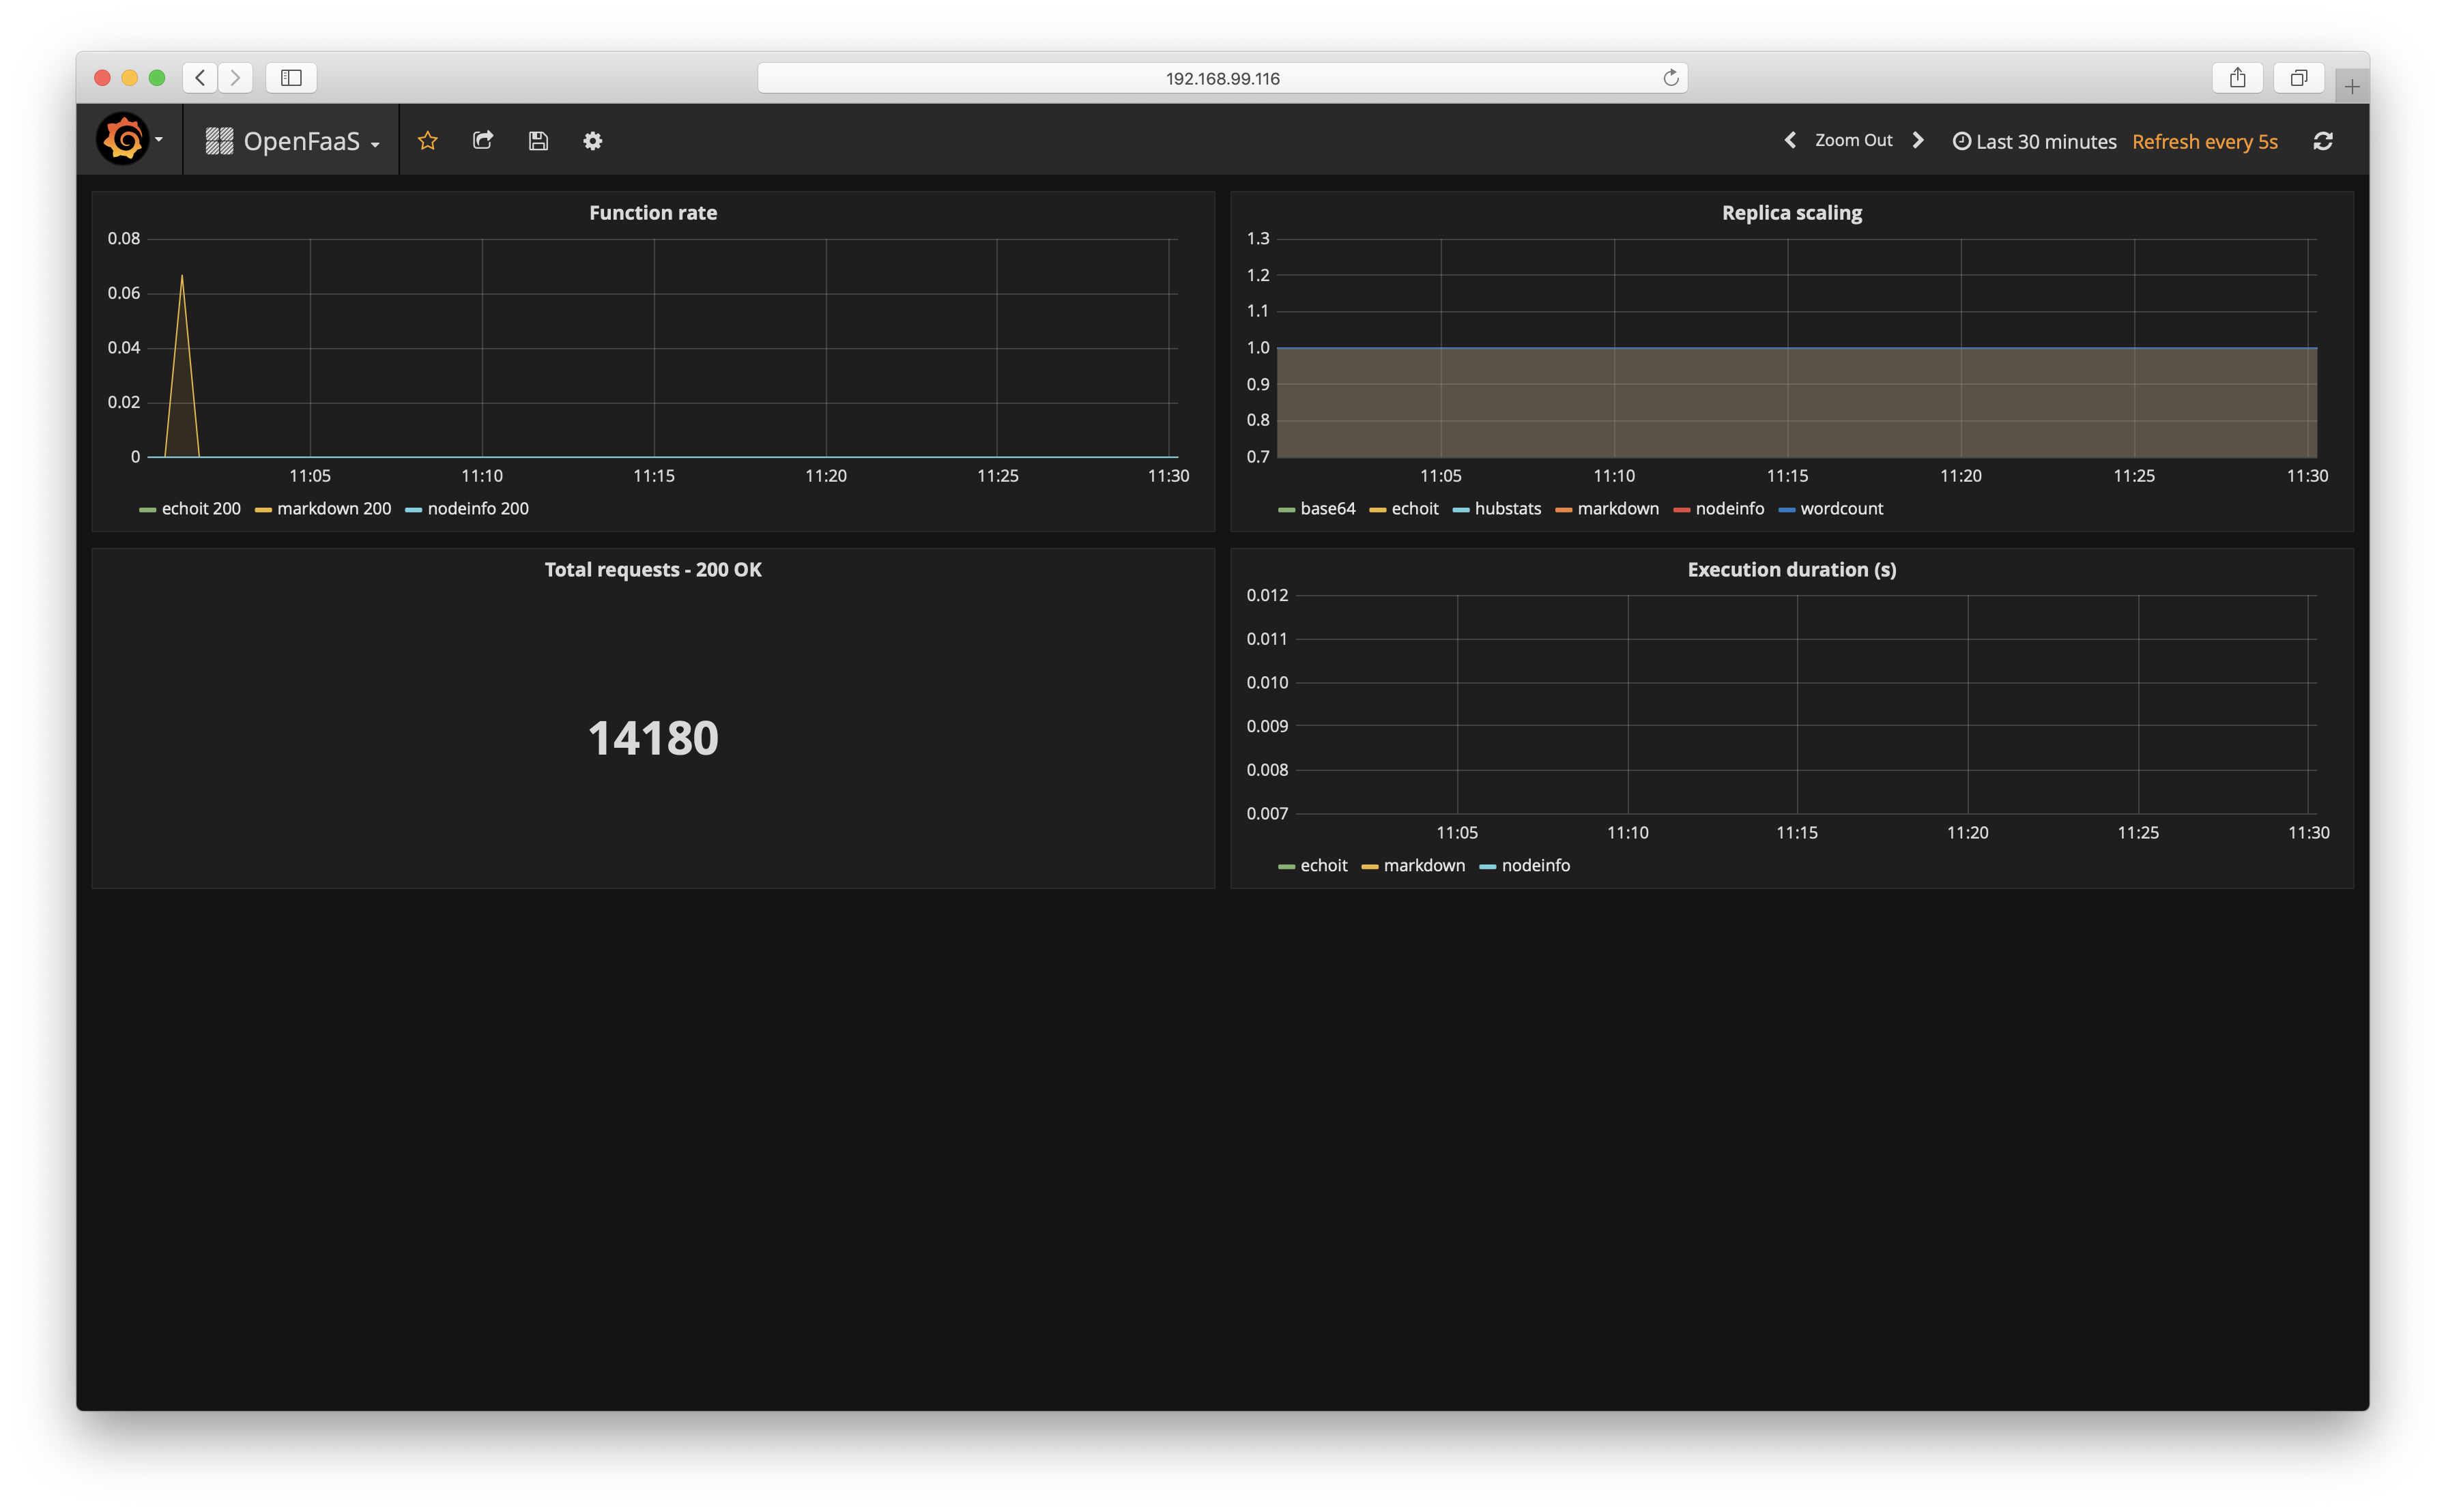
\includegraphics[width=1\textwidth]{img/grafana-dashboard.png}
    \caption{Grafana dashboard}
    \label{fig:grafana-dashboard}  
\end{figure}

\subsection{Deployment nieuwe demofunctie}
Het OpenFaaS framework wordt getest aan de hand van de zelfgeschreven functie die reeds beschreven is in sectie \ref{sec:python-demofunctie}. De functie wordt gedeployed aan de hand van de faas-cli tool. De code die werd geschreven wordt eveneens aangepast zodanig dat er gebruik kan worden gemaakt van Kubernetes secrets\footnote{https://docs.openfaas.com/reference/secrets/} voor het beheer van credentials die nodig zijn voor de Google API. Het deployen van een functie is slechts mogelijk indien alle voorgaande stappen succesvol werden uitgevoerd. Het deployen van de functie is onderverdeeld in verschillende stappen die hieronder uitgebreid worden beschreven.

\subsubsection{1. Aanmelden via faas-cli}
Indien er eerder nog niet werd ingelogd via de faas-cli dan moet dit gebeuren alvorens verder te gaan. Met behulp van volgend commando kan worden ingelogd, indien dit vanuit dezelfde shell als diegene waarin het installatiescript werd uitgevoerd gebeurt. Als de omgevingsvariabelen niet ingesteld zijn dan kunnen deze worden aangepast naar het IP adres en wachtwoord van het Tiller service account.
\begin{lstlisting}[language=bash]
$ faas-cli login -g http://$OPENFAAS_URL -u admin -p $PASSWORD
\end{lstlisting}

\subsubsection{2. Aanmaken Kubernetes secret}
Eerder werd er een credential account aangemaakt via Google Cloud API. De credentials die bij het aangemaakte account horen werden opgeslagen op een lokale locatie, deze credentials worden nu in een Kubernetes secret gestopt. OpenFaaS kan secrets uitlezen en deze gebruiken in functies, dit zorgt voor extra security, zo hoeven de credentials niet aanwezig te zijn in de Docker image van de functie.

\begin{lstlisting}[language=bash]
$ kubectl create secret generic secret-api-credentials \
 --from-file=secret-api-credentials=credentials-serverless.json \
 --namespace openfaas-fn
\end{lstlisting}

\subsubsection{3. Deploy functie}
De eerste keer dat de gebruiker een functie wilt deployen moeten er enkele stappen worden genomen, de functie moet worden geschreven, een YAML bestand met parameters specifiek voor deployment moet worden gemaakt en de gebruiker moet inloggen op Docker Hub voor het publiceren van Docker images. Wanneer een gebruiker een functie maakt, dan wordt deze op Docker Hub geplaats, vandaar het belang dat de gebruiker inlogt. Volgende stappen worden ondernomen wanneer de demofunctie voor het eerst wordt gedeployed.

\begin{lstlisting}[language=bash]
# 1. Login op Docker Hub
$ docker login

# 2. Maak een nieuwe functie
$ mkdir demo-functie; cd demo-functie

# serverless-demo is de naam die de functie zal krijgen,
# prefix is de gebruikersnaam op Docker Hub

$ faas-cli new --lang python serverless-demo --prefix="lennertmertens"

# De inhoud van de map ziet eruit als volgt na uitvoer 
# van vorig commando
$ ls
serverless-demo     serverless-demo.yml    template

# Vul de template bestanden aan naar eigen wensen en schrijf de functie
# De inhoud van de bestanden wordt hieronder weergegeven

# 3. Build de functie die werd geschreven
$ faas-cli build -f serverless-demo.yml

# 4. Push de Docker image van de functie naar Docker Hub
$ faas-cli push -f serverless-demo.yml

# 5. Deploy de functie op het OpenFaaS framework
$ faas-cli deploy -f serverless-demo.yml
\end{lstlisting}

De bestanden voor het maken en deployen van de functie zien er als volgt uit.

\subsubsection{serverless-demo.yml}
Aan de hand van dit bestand wordt de functie gedeployed. Dit bestand is een template waaraan enkele zaken zijn toegevoegd die specifiek zijn voor de demo-omgeving die werd opgezet. In bijlage \ref{sec:serverless-demo.yml} is de inhoud van dit bestand terug te vinden. De gateway is de URL van de OpenFaaS omgeving. De image is de Docker image dat wordt gebruikt voor het deployen van de functie op het framework. De ''secrets'' optie moet eveneens worden toegevoegd indien er gebruik wordt gemaakt van een Kubernetes secret, op die manier kan de functie de inhoud ervan opvragen.

\subsubsection{severless-demo/handler.py}
Onder de map serverless-demo is het handler.py bestand terug te vinden, dit is een Python script dat de functionaliteit bevat. Het Python bestand is de code die de functie vormt. In bijlage \ref{sec:demofunctie-openfaas} is de code te zien die specifiek voor deze opstelling wordt gebruikt

\subsubsection{serverless-demo/requirements.txt}
Onder de serverless-demo map is eveneens een requirements.txt bestand terug te vinden. Het bestand bevat de dependencies waar het Python script afhankelijk van is, dit zijn packages nodig om de functie uit te voeren. De packages staan opgelijst in bijlage \ref{sec:requirements.txt}.

\subsection{Deployment bestaande functie}
Wanneer de functie werd gebuild en in een repository op Docker Hub werd geplaatst dan volstaat het om enkel een template file te hebben zoals \ref{sec:serverless-demo.yml}. De functie wordt vanaf een bestaande image gedeployed dus het is niet meer nodig deze image opnieuw te builden. Images in Docker registries bieden de mogelijkheden dat ze eender waar kunnen worden gebruikt door iedereen of door een afgeschermde groep mensen. Het voordeel van serverless functies is dat er per functie een container wordt gebuild die alle dependencies en runtime voor een specifiek stuk code bevat.

\begin{lstlisting}
# Deploy bestaande functie op het OpenFaaS framework
$ faas-cli deploy -f serverless-demo.yml
\end{lstlisting}

